% New papers to check out

% @article{PhysRevA.103.032810,
%   title = {Magic wavelengths for the helium $2{\phantom{\rule{0.16em}{0ex}}}^{3}{S}_{1}\ensuremath{\rightarrow}2{\phantom{\rule{0.16em}{0ex}}}^{1}{P}_{1}$ forbidden transition},
%   author = {Zhang, Yong-Hui and Tang, Li-Yan and Zhang, Jun-Yi and Shi, Ting-Yun},
%   journal = {Phys.
	% Rev.
	% A},
%   volume = {103},
%   issue = {3},
%   pages = {032810},
%   numpages = {7},
%   year = {2021},
%   month = {Mar},
%   publisher = {American Physical Society},
%   doi = {10.1103/PhysRevA.103.032810},
%   url = {https://link.aps.org/doi/10.1103/PhysRevA.103.032810}
% }




% https://arxiv.org/pdf/2103.14365.pdf

% https://www.sciencedirect.com/science/article/abs/pii/S0009261421003237
%  doubly excited states of He
\chapter{Frequency measurements of resonances between the second and fifth manifolds in {$^4$}\mhe}
\markboth{\thechapter. TRANSITION FREQUENCY MEASUREMENTS}{}
\label{chap:transitions}

\blankfootnote{\noindent The contents of this chapter relate to the work published in \textbf{Frequency measurements of transitions from the $2\triplet P_2$ state to the $5\singlet D_2$, $5\triplet S_1$, and $5\triplet D$ states in ultracold helium} by J. A. Ross, K. F. Thomas, B. M. Henson, D. Cocks, K. G. H. Baldwin, S. S. Hodgman, A. Truscott, \href{https://journals.aps.org/pra/abstract/10.1103/PhysRevA.102.042804}{\emph{Physical Review A} \textbf{102}} (2020)}




  {The} appearance of ordinary matter arises from interactions between charged particles and light.
	This phenomenon is the domain of the theory of quantum electrodynamics (QED), which provides the most accurate quantitative predictions of any physical theory to date.
	The theory of QED is the workhorse of modern atomic structure calculations, whose only inputs are the CODATA values of three physical constants: the proton-electron mass ratio, the Rydberg constant, and the fine structure constant $\alpha$.
	These constants of nature can be constrained with state-of-the-art atomic spectroscopy, which is accurate enough to match theoretical uncertainties in table-top experiments.
	Thanks to the quality of modern theory and experiment, atomic structure measurements reprise their role in frontier tests of physics.
	
\section{Introduction}

  In 1964, Charles Schwartz proposed the determination of $\alpha$ from the fine structure intervals of the $2\triplet P$ manifold in helium, which are subject to strong QED effects \cite{Schwartz64}.
	The contemporary knowledge of helium's structure greatly exceeds Schwartz's anticipation of parts-per-million accuracy.
	For example, the $2\triplet S_1 - 2\triplet P$ and $2\triplet P - 3\triplet D$ intervals measured by Cancio Pastor \textit{et al.} \cite{Pastor04} and Luo \emph{et al.} \cite{Luo15}, respectively, both have relative uncertainties better than 50 parts per \emph{trillion}, providing Lamb shift measurements accurate to several ppm.
	The measurement of the $\PStateManifold$ fine structure splitting by Smiciklas \textit{et al.} to sub-kilohertz precision determines $\alpha$ to several ppb \cite{Smiciklas10}.
	Measurements of the $2^{3\!}P_1-2^{3\!}P_2$ interval by Kato \emph{et al.}, accurate to 25Hz, would constrain $\alpha$ to less than one ppb given a similarly accurate measurement of the $2^{3\!}P_0 - 2^{3\!}P_1$ transition and QED calculations including terms of order $\alpha^7$ \cite{Kato18}.
	

  \begin{figure}
  	
  	\begin{minipage}[t]{0.38\textwidth}
			\vspace{0pt}
      \caption{Energy level diagram for $^4$He showing the transitions measured in this work (blue) are driven by a tunable laser referred to in the text as the \emph{probe beam}.
				A laser tuned to the $2\triplet S_1-2\triplet P_2$ transition (red, referred to as \emph{pump beam}) populates the lower state of the target transitions.
				 The doubly forbidden $1^{1\!}S_0 - 2^{3\!}S_1$ transition is excited in a high voltage discharge source.
				Transitions across the dotted line are \emph{forbidden} by the $\Delta S=0$ selection rule.
				Level splittings are not to scale.}
      \label{fig:lvl_diag}
      \end{minipage}
      \hfill
      \begin{minipage}[t]{0.6\textwidth}
      \vspace{0pt}
      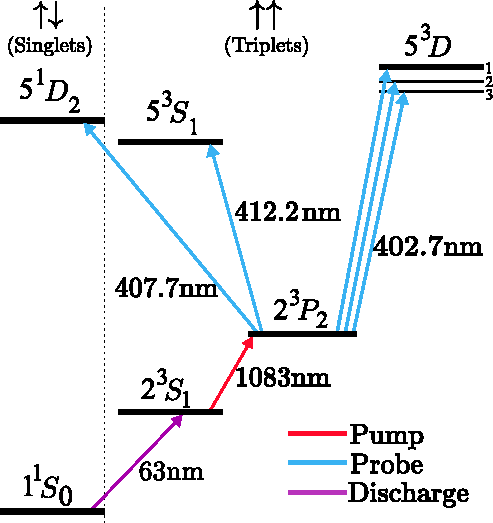
\includegraphics[width=\textwidth]{fig/spectroscopy/level-diagram-tight-latex-pdf.pdf}
      \end{minipage}
  \end{figure}

  A concurrent issue is the so-called `proton radius puzzle': Determinations of the proton charge radius from Lamb shift measurements in muonic and electronic hydrogen \cite{Pohl10, Bezginov19}, electron-hydrogen scattering experiments \cite{Beyer17,Xiong19}, and isotope shifts in light muonic atoms \cite{Kalinowski19,Pohl16} disagree significantly with both the CODATA recommended value and with other recent experiments \cite{Fleurbaey18}.
	 Helium is a promising candidate to provide insight into this unresolved issue because its simple structure is tractable to QED calculations.
	Furthermore, ongoing theoretical work \cite{Pachucki15,Pachucki17,Pachucki11,Pachucki10,Morton12,Morton06,Patkos16,Patkos17} and recent high-precision measurements \cite{Rooij11,Notermans14,Notermans16,Rengelink18} find a $4\sigma$ discrepancy between the difference $\delta = r^2(^3\textrm{He}) - r^2(^4\textrm{He})$ of squared nuclear charge radii obtained from the isotope shifts of the $\MetastableState - \PStateManifold$ and ${2^{1\!}S_{0}} - \MetastableState$ transitions \cite{Pachucki15,Patkos17}.
	The completed calculation of QED effects to order $\alpha^7$ will allow determination of the absolute nuclear charge radii accurate to better than 1\% \cite{Pachucki17}.
	Along with these $\alpha^7$ contributions, measurement of the $2\triplet S-2\triplet P$ spacing to within 1.4 kHz would allow a determination of the nuclear charge radius to below 0.1\% accuracy, better than expected from the muonic helium Lamb shift \cite{Wienczek19}.
	The corresponding QED calculations to seventh order have been completed (Ref. \cite{Patkos21}) since the publication of the work in this chapter. 
	The authors note, however, that the predicted energies of the $2\triplet S - 3 \triplet D$ and $2\triplet P - 3 \triplet D$ transitions disagree significantly with experiments, and refrain from computing the nuclear charge radius until these discrepancies are resolved.
	 
  Notable among recent studies of helium's structure are the measurements of \emph{forbidden} transitions between the singlet and triplet manifolds.
	Such transitions are made possible in reality due to relativistic effects and are extremely narrow, therefore precise measurements of their spectral features can provide stringent tests of QED \cite{Lach01}.
	The work in this chapter complements existing measurements of forbidden lines in helium at 1557 nm \cite{Rooij11,Rengelink18}, 887 nm \cite{Notermans14}, and 427 nm \cite{Thomas20}.

	This chapter concerns frequency measurements of the transitions from the $2^3P_2$ state to five states in the $n=5$ manifold of $^4$He, illustrated in Fig.
	\ref{fig:lvl_diag}.
	These measurements improve on the precision of previous measurements by at least an order of magnitude \cite{Martin60}, and resolve the fine structure splitting of the $\PStateManifold_2 - 5\triplet D$ transition for the first time.
	The results also include the first direct measurement of the spin-forbidden $2^{3\!}P_2 - 5^{1\!}D_2$ transition in helium, whose transition rate is four orders of magnitude smaller than the other transitions discussed here.  
	Theoretical transition energies agree with the observed values within our experimental uncertainty.

\section{Measurement technique}

	The experimental sequence began with $\sim10^8$ atoms in the metastable $2\triplet S_1$ state, cooled to  $\sim1~\textrm{mK}$ in a magneto-optical trap, which were then transferred to a magnetic trap by switching off the light.
	Next, during the Doppler cooling stage, we illuminated the atoms with $\sim$30$\mu$W$/m^2$ of $\sigma^+$ polarized cooling light, further cooling the atoms to $\sim200~\mu \textrm{K}$.
	Finally, forced evaporative cooling lowers the sample below the critical temperature to form a BEC.
	Each iteration of this procedure produced a BEC of $\sim 5\times10^5$ atoms in a cigar-shaped harmonic trap with trapping frequencies $\omega = 2\pi (425,425,45)$ Hz.
	To perform the absorption measurements, we disturbed the Doppler cooling stage by applying a probe beam tuned near the target transition, resulting in a reduction in the number of atoms cooled to degeneracy. 
	

	At the end of the experimental sequence a pulsed atom laser, described in section \ref{sec:atomlaser}, transfers $\approx$2\% of the trap population at a time to the untrapped $m_J=0$ state \cite{Manning10,Henson18_BCR}.
	The resulting coherent matter-wave pulses fall onto the detector, {depleting the entire trapped population after $\sim$200 pulses over 2 seconds.
	This allows}  the atom number and temperature to be accurately determined without saturating the detector.
	Our data collection protocol consisted of a cycle of one calibration shot (with the probe beam switched off), followed by one measurement shot (with the probe beam on simultaneously with the Doppler cooling light) at each of two magnetic field strengths used in the in-trap cooling stage.
	We denote the atom number measured at the end of the calibration and measurement shots as $N_c$ and $N$, respectively.
	The signal is defined to be the normalized loss of atoms, in the form $(N_c-N)/N_c$.
	The reference population $N_c$ was estimated by linear interpolation between the successive calibration shots either side of a given measurement shot in order to compensate for drift in the trap population over time.
	
	The physical basis of the measurement is the sensitivity of forced evaporative cooling to the initial conditions of the helium atoms.
	The precise effect of photon scattering on the final cloud properties depends on the exact details of the evaporation sequence, and is hard to model exactly.
	Instead, what follows is a qualitative picture of the role evaporative cooling plays in transforming photon scattering to a measurable change in trap population.

	During the Doppler cooling stage of BEC creation, the 1083 nm cooling beam acts as an optical pump and excites atoms to the $2\triplet P_2(m_J=2)$ state.
	From the $2\triplet P_2$ state they may decay, with a lifetime of $\sim$97ns, back to the trapped metastable state or absorb photons from the probe beam and become excited again to the target state.
	Doubly-excited atoms may decay back to the trapped $m_J=+1$ state of the $2\triplet S_1$ level, in which case the photon absorption and emission events add heat to the cloud by imparting a nonzero average impulse to the atoms.
	This leads to an initially hotter cloud, which in turn reduces the efficiency of evaporative cooling, resulting in a higher atom loss during evaporation and a lower final number in the trap. Alternatively, atoms may decay to other untrapped magnetic states of the metastable state, or to the true ground state via a spin-flip transition to the singlet manifold.

	Decay to untrapped states reduces the initial atom number and can even impart heat to the cloud as these atoms leave the trap - via scattering with trapped atoms.
	This heating will be much smaller than in the previous case because the scattering rate will be small in such a dilute gas.
	However, reducing the initial trap population also manifests as a reduced final atom number.
	In both cases the effect of photon scattering manifests as a reduction of the total trapped final number $N$ relative to the final number $N_c$ in the calibration shots.

\begin{figure}
      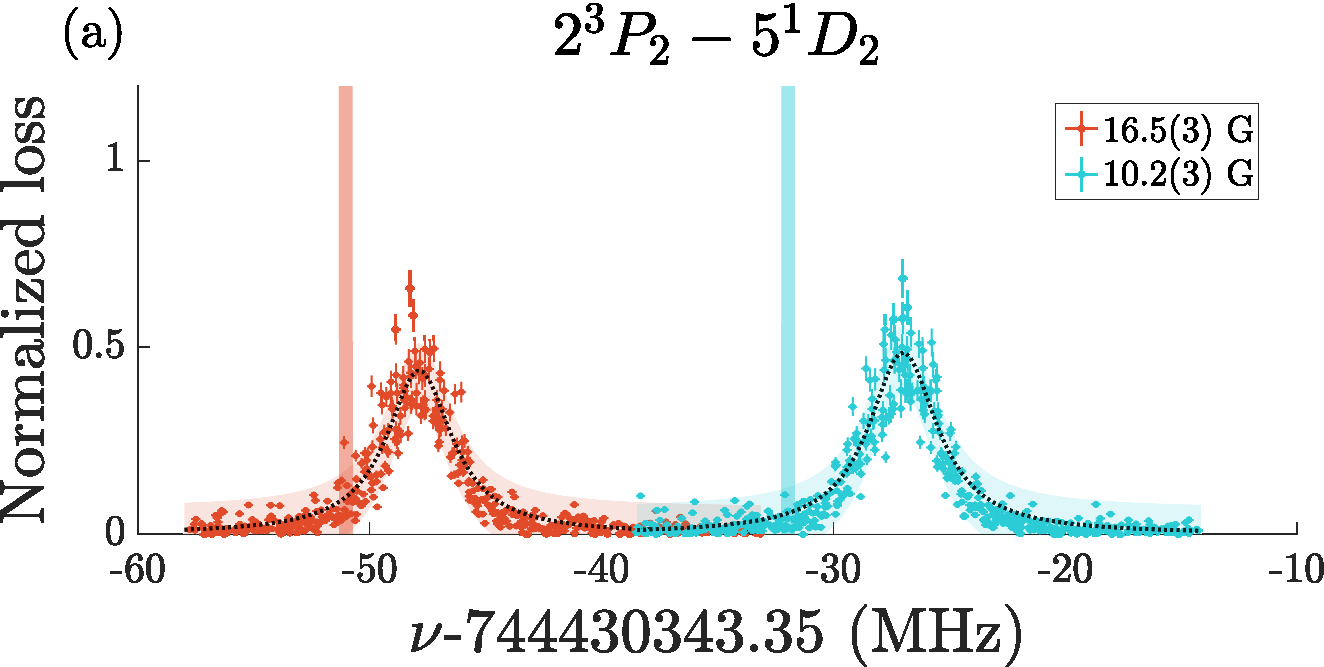
\includegraphics[width=\textwidth]{fig/spectroscopy/ci-plot-51D2.pdf}
    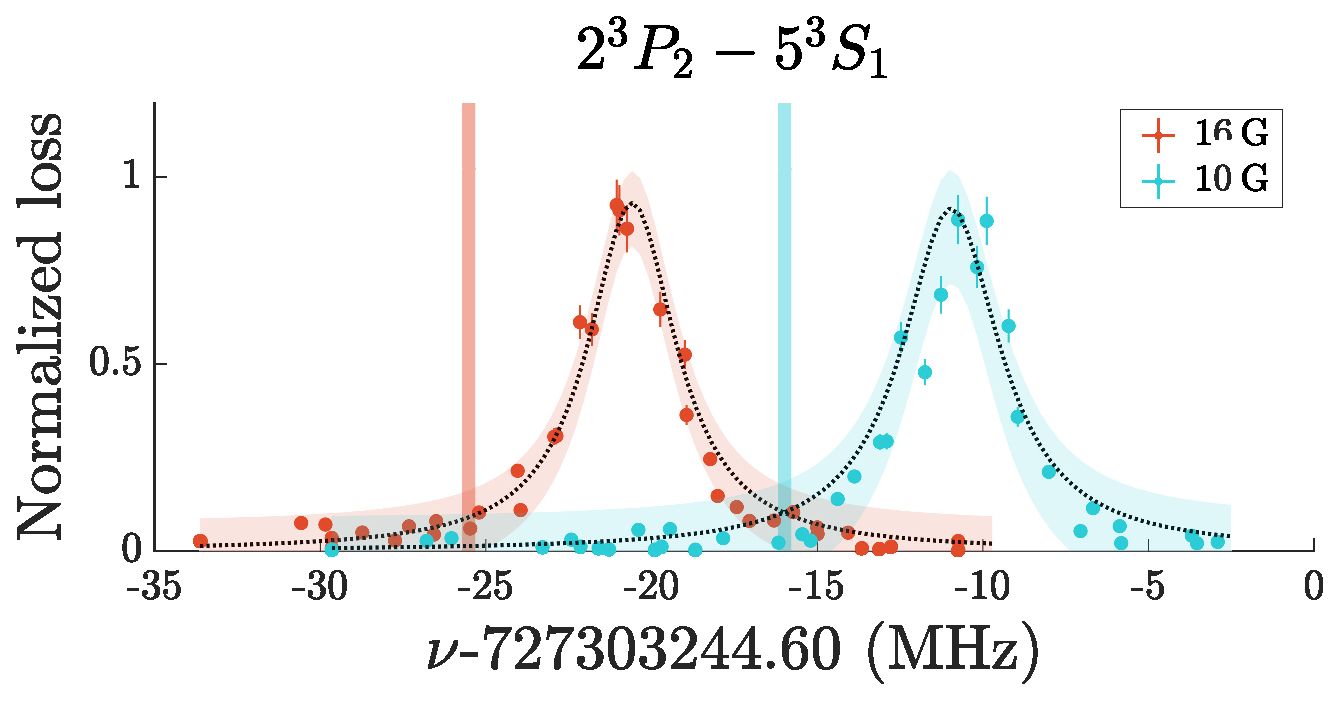
\includegraphics[width=\textwidth]{fig/spectroscopy/ci-plot-53S1}
   \caption{Line profile for (a) the spin-forbidden $\PStateManifold_2 -  5^{1\!}D_2$  and (b) the $2\triplet P_2 - 5\triplet S_1$  resonances, showing normalized atom number loss versus probe laser frequency $\nu$, as measured in a {16.5(3)} G (red) and {10.2(3)} G (blue) background field, with Lorentzian fits (black dotted line, with the observation interval shaded - see also section \ref{sec:fitting}).
	Error bars account for detector efficiency and calibration model uncertainty. 
	Vertical bars indicate theoretical predictions for the line centres, with the uncertainty (mostly due to uncertainty in the magnetic field) indicated by the width of the bars.
	For comparison, theoretical predictions (vertical bars) Zeeman shifted from the predicted zero-field value \cite{Drake07} according to the field calibration, whose uncertainty (shaded width) is dominated by background field measurements.}
    \label{fig:simple_lines}

\end{figure}


% \begin{figure}
%     \centering
%     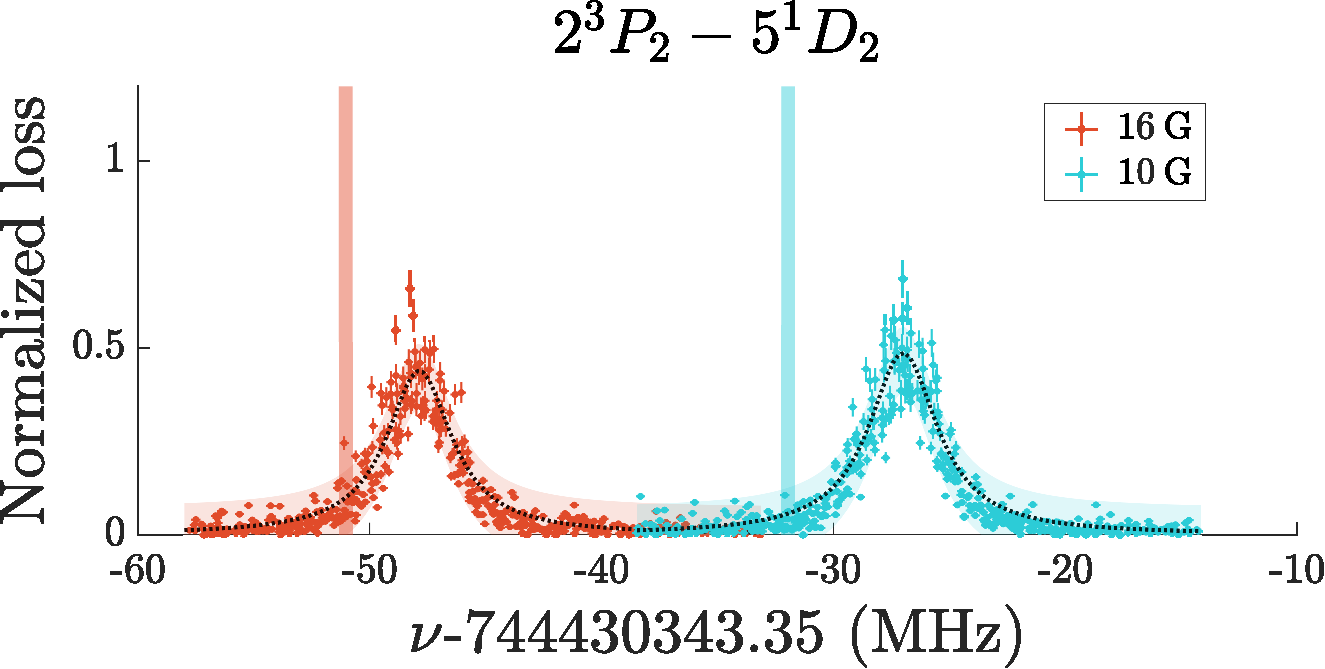
\includegraphics[width=0.66\textwidth]{fig/spectroscopy/ci-plot-51D2-eps-converted-to.pdf}
%     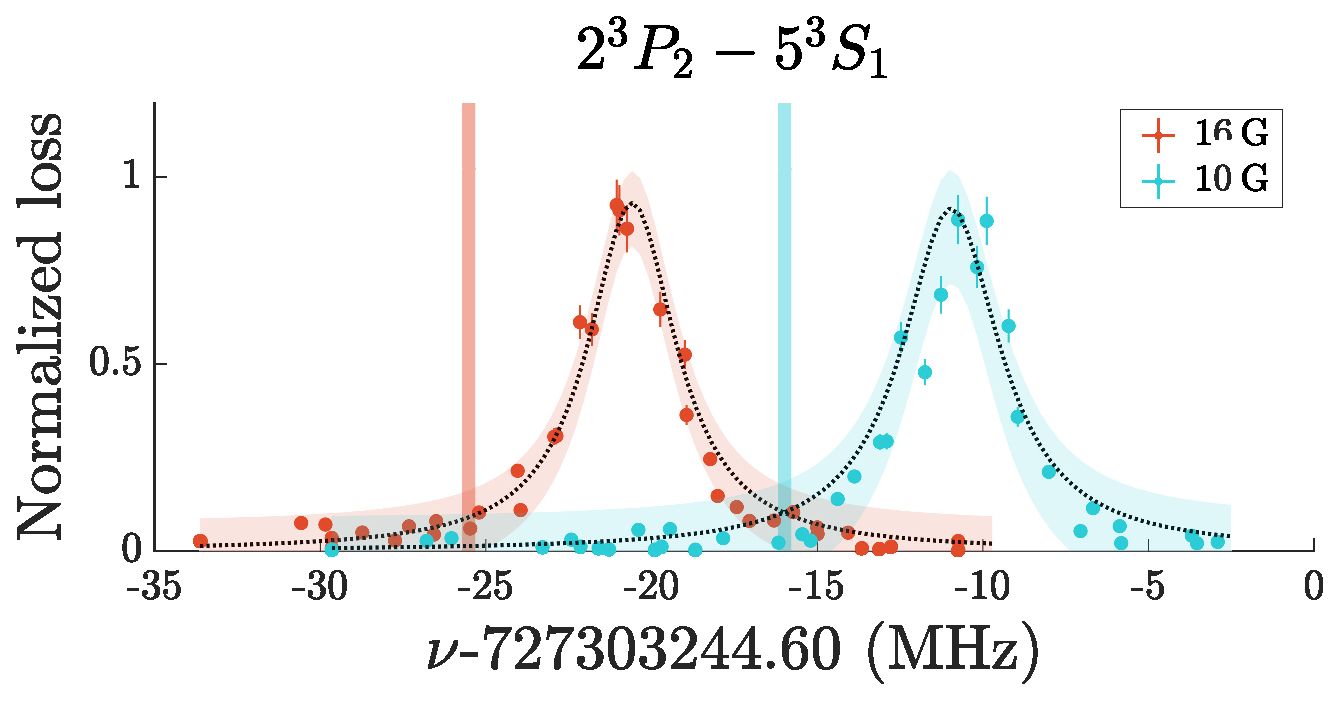
\includegraphics[width=0.66\textwidth]{fig/spectroscopy/ci-plot-53S1}
%     \caption{Line profile for the spin-forbidden $\PStateManifold_2 -  5^{1\!}D_s2$ and the $2\triplet P_2 - 5\triplet S_1$ resonances, showing normalized atom number loss versus probe laser frequency $\nu$, as measured in an {16.8(1)}G (red) and {10.06(7)}G (blue) background field, with Lorentzian fits (black dotted line, with prediction confidence interval shaded).
% 	Error bars account for detector efficiency and calibration model uncertainty.
% 	For comparison, theoretical predictions (vertical bars) Zeeman shifted from the predicted zero-field value \cite{Drake07} according to the field calibration, whose uncertainty (shaded width) is dominated by background field measurements.}
%     \label{fig:simple_lines}
%   \end{figure}


% Laser
	

	We illuminated the atoms with the probe light (generated by the system described in section \ref{sec:spec_laser}) during the Doppler cooling stage, then measured the relative number loss as a function of frequency.
	For the $5\singlet D_2$ and $5\triplet S_1$ states, the exposure time was of order 100 ms. 
	The exact duration differed for each line to obtain a good SNR without saturating the atom loss.
	The light was $\sigma^-$ polarized to drive transitions to the $m_J=1$ states of the upper levels.
	For the forbidden $5\singlet D_2$ transition the beam was focused on the atom cloud with a waist of approximately $100~\mu$m and a peak intensity of order $5\times 10^3$ W/m$^2$.
	For all other measurements the beam was collimated with a peak intensity of order $ 5$ W/m$^2$.
	The Doppler cooling stage uses two magnetic field strengths and so measurements could be made with bias field strengths of {16.5(3)} and {10.2(3)} Gauss, which were calibrated independently by RF spectroscopy.
	For each field strength, the atom loss (with respect to calibration shots) versus probe laser frequency can be fitted by a Lorentzian lineshape to obtain the centre frequency and full-width at half-maximum (FWHM).
	Results of these measurements are shown in Tab.	\ref{fig:simple_lines}, after corrections for the AOM and vapor cell shifts (see the supplementary material of \cite{Thomas20} for details on the latter).
	The functional relationship between photon scattering and atom loss via evaporative cooling is complicated and not linear. 
	However, fits using a nonlinear function of the Lorentzian lineshape differed from the simple Lorentzian fit by substantially less than the statistical uncertainty.
	It would be interesting to study the relationship between the signal strength and photon scattering rate as a means to measure the oscillator strength of these transitions.
	This study would also need to characterize the population of the $2\triplet P_2$ in response to the probe beam. One approach would be to start by constructing a model of this intermediate process. It would be necessary to anchor this model to empirical reality, which may not be straightforward.

	After correcting for the linear Zeeman shift, the field-free transition frequencies are fixed with sub-MHz statistical uncertainty.
	This determines the $2\triplet P_2-5\singlet D_2$ and $2\triplet P_2-5\triplet S_1$ transition energies to be 3 MHz and 5 MHz larger, respectively, than the predictions presented in \cite{Drake07}.
	However, the absolute accuracy of these measurements is limited by the instrumentation.
	The results (Tab.	\ref{tab:spec_results}) are consistent with current predictions \cite{Drake07} within $2\sigma$ after accounting for all systematic uncertainties (Tab.	\ref{tab:errors}).
	%mark




\section{5$\triplet$D fine structure}

	Unlike the $5\singlet D_2$ and $5\triplet S_1$ levels, the $5\triplet D$ manifold splits into fine structure sublevels, leading to multiple absorption peaks and requiring a more involved analysis.
	For this measurement, the final quarter-wave plate in the insertion optics was rotated to give a combination of $\pi$ and $\sigma^-$ polarized light (in the atomic frame) as opposed to pure $\sigma^-$ light.
	This light drove transitions to the $5\triplet D_J, J\in\{1,2,3\}$ levels and obtained four peaks, as shown in Fig.	\ref{fig:combined_5D_lines}.
	The saturated peak near -300 MHz (relative to the predicted $2\triplet P_2 - 5\triplet D_1$ interval) is in fact two peaks corresponding to the $5\triplet D_2(m_J=1)$ and $5\triplet D_3(m_J=2)$ states, which are separated by less than their linewidth. These peaks are excluded from the analysis below.
	This illustrates a shortcoming of the technique, namely the limited dynamic range.
	Specifically, that the sensitivity (roughly, the smallest detectable signal from a given number of measurements) is limited by the shot noise (the shot-to-shot variation) in atom number, whereas the maximum detectable signal is one that completely depletes the condensate. Therefore, when two peaks are close by, they both contribute to absorption and if they would otherwise individually deplete most of the condensate, their combined absorption peak will be saturated.

	For measurements of single peaks this is not an issue as the total irradiated energy can be adjusted to obtain a good signal-to-noise ratio without completely depleting the BEC.
	In this case, however, there is a trade-off between keeping the small peaks above the noise floor and preventing the superposed peaks from saturating.
	This limitation could be eased with a larger initial condensate because the dynamic range is essentially limited by the atom loss, with much larger magnetic field strengths which would ensure the lines are separated by much more than their linewidth, or by measuring the neighbouring peaks separately with a lower laser intensity (the cost of reduced accuracy in fitting the better-distinguished peaks could be recouped by the present measurement). 
	The other peaks correspond to transitions to the $5\triplet D_2(m_J=2)$, $5\triplet D_2(m_J=1)$, and $5\triplet D_1(m_J=1)$ states, which are used in the analysis described below.

	The Zeeman shift of the $J=2$ and $J=3$ levels is comparable to the interval between them, and so the mixing of levels means the correction is no longer proportional to $B$.
	Instead, the Zeeman shift can be corrected for by solving the eigenvalue optimization problem 
%
\begin{equation}
\textrm{min}_{E_{\textrm{fs}}} \sum_{J,m_J} \left(\nu_{{J,m_J}}^{\textrm{{pred}}}(E_{\textrm{fs}},B) - \nu_{{J,m_J,B}}^{\textrm{{obs}}}\right)^2,
\label{eqn:opt-problem}
\end{equation}
%
which minimizes the squared error between observed and predicted transition frequencies ($\nu^{\textrm{{obs}}}$ and $\nu^{{\textrm{pred}}}$ respectively), summed over all relevant $|J,m_J\rangle$ states and magnetic field strengths $B$.
	The optimized variable $E_{\textrm{fs}}=(E_1,E_2,E_3)$ is the bare fine-structure splitting of the $5\triplet D$ levels.
	In the argument below, the only assumption is the formalism of atomic structure theory and the data from the experiment.
	To determine the bare $5\triplet D$ transition energies from the data, consider the Hamiltonian
%
\begin{equation}
    \hat{H}(B) = \hat{H}_{\textrm{fs}} - B\hat{\mu}_z,
    \label{eqn:hamiltonian}
\end{equation}
%

\begin{figure}
	\centering
	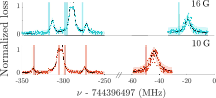
\includegraphics[width=\textwidth]{fig/spectroscopy/ci-plot-53D}
   \caption{Line profiles for the $\PStateManifold_2 -  5^{3\!}D$ transitions, shown as for Fig.
	\ref{fig:simple_lines}.
	The normalized loss is shown versus probe laser frequency for the two different field strengths with a common horizontal scale.
	Theory lines indicate predictions from \cite{Drake07} after applying the relevant Zeeman shift.
	N.B.	the scale break here and in Fig.	\ref{fig:fitting_3D} coincide.}
    \label{fig:combined_5D_lines}
\end{figure}

% \begin{figure}
%   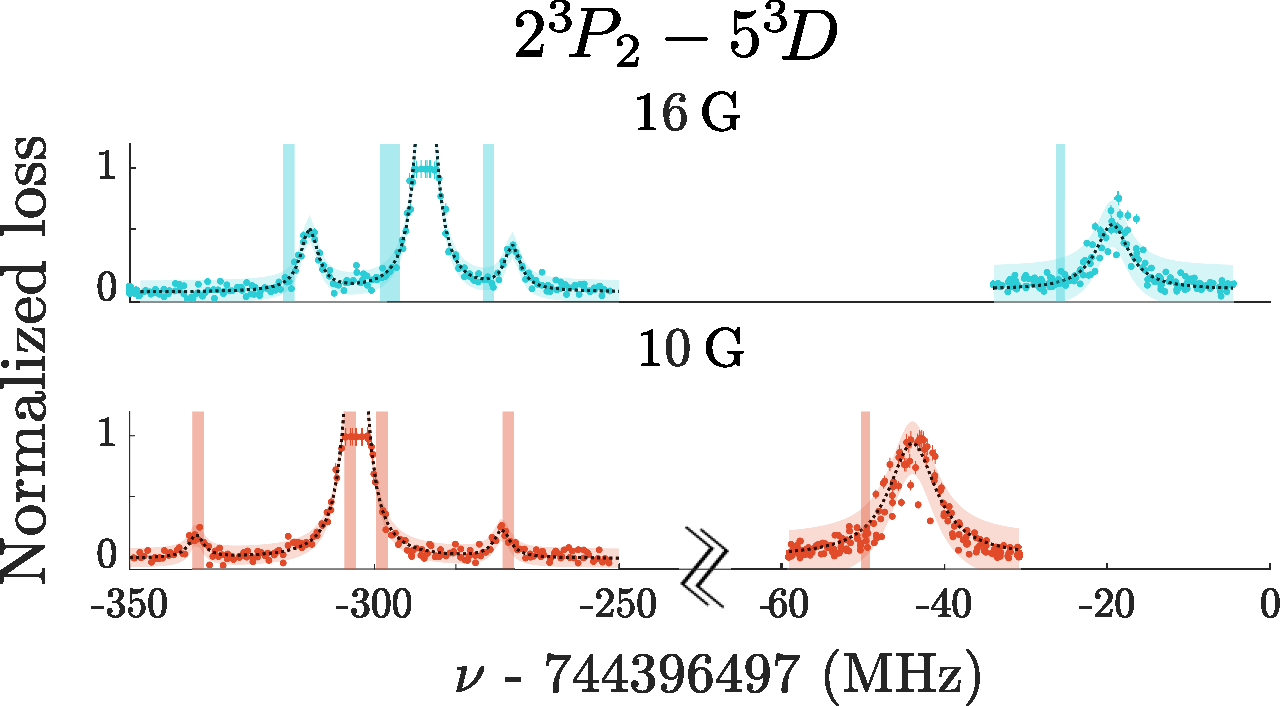
\includegraphics[width=0.5\textwidth]{fig/spectroscopy/ci-plot-53D-eps-converted-to.pdf}
%   \caption{Line profiles for the $\PStateManifold_2 -  5^{3\!}D$ transitions, shown as for Figs.
% 	\ref{fig:simple_lines}.
% 	The normalized loss is shown versus probe laser frequency for the two different field strengths with a common horizontal scale.
% 	Theory lines indicate predictions from \cite{Drake07} after applying the relevant Zeeman shift.
% 	N.B.	the scale break here and in Fig.	\ref{fig:fitting_3D} coincide.}
%   \label{fig:combined_5D_lines}
% \end{figure}

%
	\noindent where $\hat{\mu}_z = \mu_B(\hat{L}_z + g_s \hat{S}_z)/\hbar$ is the coupling of the orbital and spin angular momenta of the electron with a magnetic field of strength B pointing in the $z$-direction, $\mu_B$ is the Bohr magneton and $g_s$ is the electron spin $g$-factor.
		The fine structure Hamiltonian $\hat{H}_{\textrm{fs}}$ is diagonal in the $|LSJ m_J\rangle$ basis with eigenvalues $E_{\textrm{fs}}$,
	%
	\begin{equation}
	  \hat{H}_{\textrm{fs}}|LSJm_J\rangle = E_{\textrm{fs},LSJ}|LSJm_J\rangle,
	\end{equation}
	%
	which are degenerate for all $m_J$ with fixed $J$.
		The magnetic moment $\hat{\mu}_z$ couples states of different $J$, and is instead diagonal in the $|L m_L S m_S\rangle$ basis.
		In the $|LSJ m_J\rangle$ basis the matrix elements of $\hat{H}(B)$ are, with abbreviated notation,
	%
	\begin{equation}
	\begin{aligned}
	H_{J',J} =& \langle J'|\hat{H}|J \rangle\\
	  =& E_{\textrm{fs},J} - B \frac{\mu_B}{\hbar} \sum_{m_L} (2m_J - m_L)C_{J,'m_L}C_{J,m_L},\\
	\end{aligned}
	\end{equation}
	%
	where $C_{J,m_L} = \langle LSJ m_J|L m_L S m_S\rangle$ is shorthand for the Clebsch-Gordan coefficients.
		For $B>0$, the contribution of $\hat{\mu}_z$ breaks the degeneracy of $\hat{H}_{\textrm{fs}}$, giving rise to the Zeeman shift.
		
	%
	%
	\begin{figure}
	\centering
		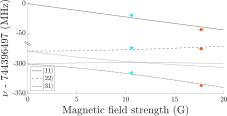
\includegraphics[width=0.9\textwidth]{fig/spectroscopy/fitting-lines}
		\caption{Determining the $5\triplet D$ fine-structure splitting.
		The values for the $|J,m_J\rangle=5\triplet D_J(m_J)$ levels (grey lines) at $B=0$ are fixed by solving the optimization problem (Eqn.
		\ref{eqn:opt-problem}), constrained by the fitted peak centres (filled circles).
		The saturated peaks are not used to constrain the levels and are not shown here. \com{}
		The corresponding frequencies predicted by the optimization method are shown in dotted lines.}
	    \label{fig:fitting_3D}
	\end{figure}

	The solution of Eqn.
	\ref{eqn:opt-problem} is illustrated in Fig.
	\ref{fig:fitting_3D}.
	By defining the energies $E_{\textrm{fs}}$ relative to the $2\triplet P_2(m_J=2)$ state,  the predicted transition frequencies can be read directly from the eigenvalues of $\hat{H}$ via $\nu_{J,m_J}^{\textrm{pred}}=E_{J,mJ}(B)/h$, where $h$ is Planck's constant.
	The observed frequencies $\nu_{J,m_J,B}^{\textrm{obs}}$ used in this procedure exclude the overlapping saturated peaks because their centre frequencies cannot be determined with satisfactory accuracy.
	The triple $E_{\textrm{fs}}$ which minimizes the cost function (Eqn.
	\ref{eqn:opt-problem}) corresponds to the $2\triplet P_2 - 5\triplet D_J$ intervals at $B=0$, as listed in Tab.
	\ref{tab:spec_results}.
	Again, the difference in this determination of the field-free splitting is consistent within 2$\sigma$ predictions in \cite{Drake07} after accounting for systematic effects (Tab.
	\ref{tab:errors}).
	


% \usepackage{floatrow}



% \begin{figure}
% \floatbox[{\capbeside\thisfloatsetup{capbesideposition={left,top},capbesidewidth=4cm}}]{figure}[\FBwidth]
% {\caption{A test figure with its caption side by side}\label{fig:test}}
% {\includegraphics[width=5cm]{name}}
% \end{figure}

% \begin{figure}
% \floatbox[{\capbeside\thisfloatsetup{capbesideposition={right,top},capbesidewidth=4cm}}]{figure}[\FBwidth]
% {\caption{A test figure with its caption side by side}\label{fig:test}}
% {\includegraphics[width=5cm]{name}}
% \end{figure}




% \begin{figure}
% 	\begin{minipage}[t]{0.38\textwidth}
% 			\vspace{0pt}
% 			\caption{Determining the $5\triplet D$ fine-structure splitting.
% 	The values for the $|J,m_J\rangle=5\triplet D_J(m_J)$ levels (grey lines) at $B=0$ are fixed by solving the optimization problem (Eqn.
% 	\ref{eqn:opt-problem}), constrained by the fitted peak centres (filled circles).
% 	The saturated peaks are not used to constrain the levels, but are shown with hollow circles and the corresponding frequencies predicted by our method are shown in dotted lines.}
%     \label{fig:fitting_3D}
% 	\end{minipage}\hfill
% 	\begin{minipage}[t]{0.6\textwidth}
% 		\vspace{0pt}
% 		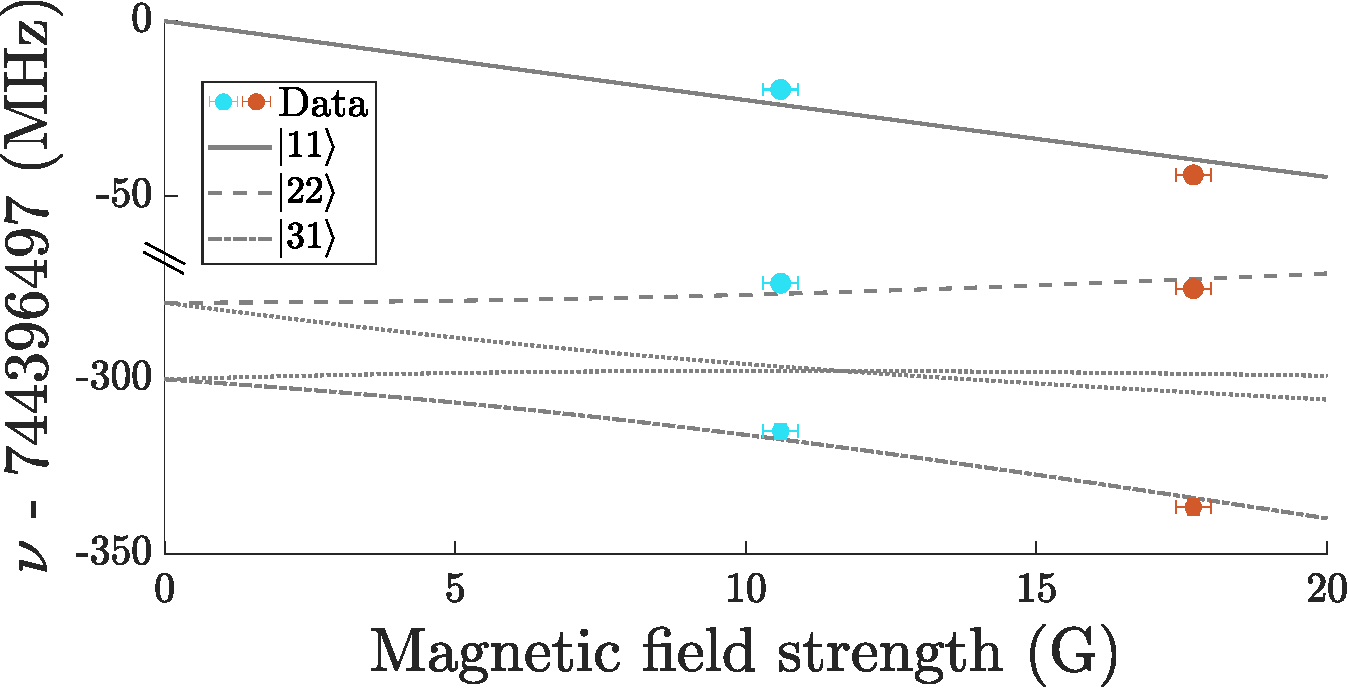
\includegraphics[width=\textwidth]{fig/spectroscopy/fitting-lines-eps-converted-to.pdf}
% 	\end{minipage}

% \end{figure}

% \begin{figure}
%     \centering
%     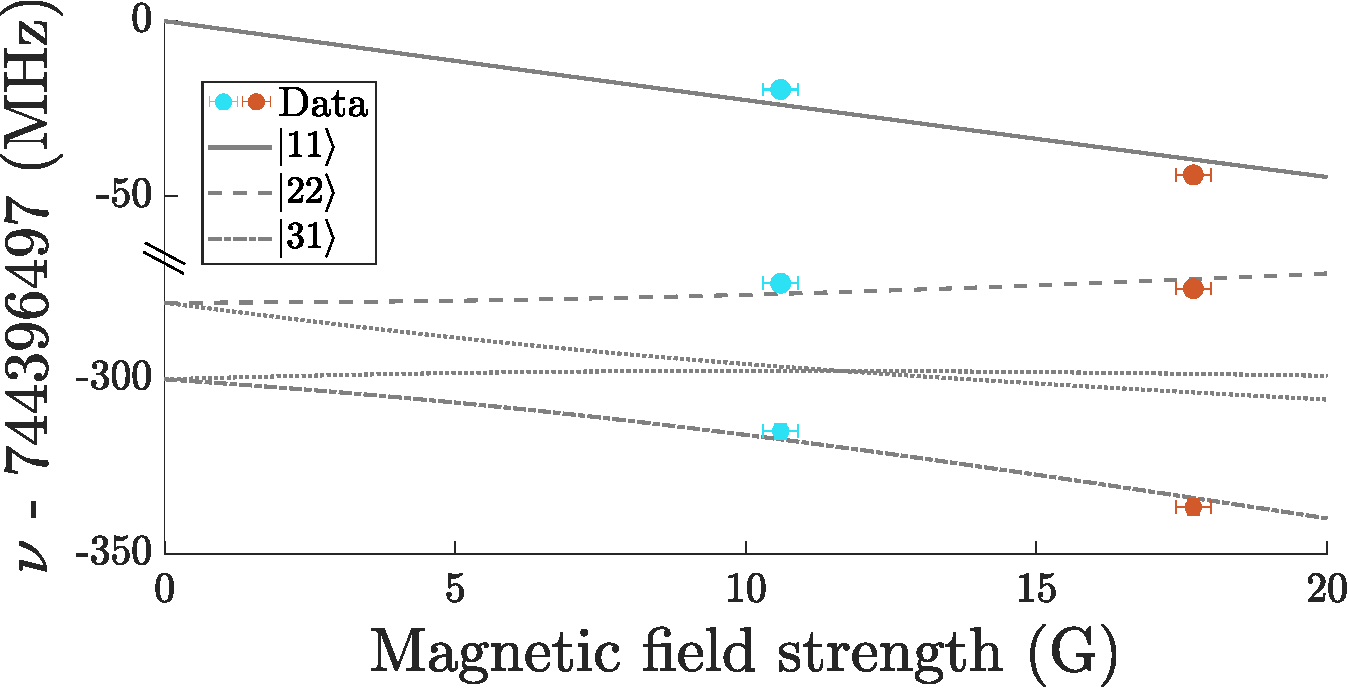
\includegraphics[width=0.48\textwidth]{fig/spectroscopy/fitting-lines-eps-converted-to.pdf}
%     \caption{Determining the $5\triplet D$ fine-structure splitting.
% 	The values for the $|J,m_J\rangle=5\triplet D_J(m_J)$ levels (grey lines) at $B=0$ are fixed by solving the optimization problem (Eqn.
% 	\ref{eqn:opt-problem}), constrained by the fitted peak centres (filled circles).
% 	The saturated peaks are not used to constrain the levels, but are shown with hollow circles and the corresponding frequencies predicted by our method are shown in dotted lines.}
%     \label{fig:fitting_3D}
% \end{figure}



\begin{table*}
\centering
  % \begin{tabular}{c c c c c c c c c c c}
  %     \hline\hline
  %     Transition                        & &  $f_\textrm{exp}$ & &  $f_\textrm{theory}$ & Ref.
		% &  $f_\textrm{exp}-f_\textrm{theory}$      & &  $\textrm{FWHM}_{\textrm{exp}}$  & &  $\textrm{FWHM}_{{\textrm{pred}}}$ \\
  %     \hline
  %       $2\triplet P_2 - 5^3\mathrm{S}_1$ & &  {727,303,248(3)} & &  727,303,244.6(4)   & \cite{Drake07} &  {3(3)}    & &  3.4(5)  & &  1.5\\ % A = 
  %       $2\triplet P_2 - 5^3\mathrm{D}_1$ & &  {744,396,496(7)} & &  744,396,511.1(7)   & \cite{Yerokhin20} &  {-16(7)}    & &  5.8(6)  & &  2.6\\
  %       $2\triplet P_2 - 5^3\mathrm{D}_2$ & &  {744,396,220(7)} & &  744,396,227.6(7)   & \cite{Yerokhin20} &  {-8(7)}    & &  4.2(5)  & &  2.6\\
  %       $2\triplet P_2 - 5^3\mathrm{D}_3$ & &  {744,396,194(7)} & &  744,396,208.3(7)   & \cite{Yerokhin20} &  {-14(7)}    & &  4.0(1)  & &  2.6\\
  %       $2\triplet P_2 - 5^1\mathrm{D}_2$ & &  {744,430,343(7)} & &  744,430,343.1(7)   & \cite{Yerokhin20} &  {0(7)}    & &  3.2(1)  & &  2.2\\  % 744430344
  %     \hline\hline
  %   \end{tabular}

    \begin{tabular}{c c c c c c c c c c c}
      \hline\hline
      Transition                        &  $f_\textrm{exp}$ &  $f_\textrm{theory}$ & Diff.
		  &  $\textrm{FWHM}_{\textrm{exp}}$  &  $\textrm{FWHM}_{{\textrm{pred}}}$ \\
      \hline
        $2\triplet P_2 - 5^3\mathrm{S}_1$ &  {727,303,248(3)} &   727,303,244.6(4)   &  {3(3)}      &  3.4(5)  &  1.5\\ % A = 
        $2\triplet P_2 - 5^3\mathrm{D}_1$ &  {744,396,496(7)} &   744,396,511.1(7)   &  {-16(7)}     &  5.8(6)  &  2.6\\
        $2\triplet P_2 - 5^3\mathrm{D}_2$ &  {744,396,220(7)} &   744,396,227.6(7)   &  {-8(7)}      &  4.2(5)  &  2.6\\
        $2\triplet P_2 - 5^3\mathrm{D}_3$ &  {744,396,194(7)} &   744,396,208.3(7)   &  {-14(7)}     &  4.0(1)  &  2.6\\
        $2\triplet P_2 - 5^1\mathrm{D}_2$ &  {744,430,343(7)} &   744,430,343.1(7)   &  {0(7)}      &  3.2(1)  &  2.2\\  % 744430344
      \hline\hline
    \end{tabular}
\caption{Summary of results for each transition.
	After correcting for the AOM and vapor cell shifts, the centre frequencies obtained from Lorentzian fits have statistical error at the 10 kHz level.
	The field-free energies follow after correcting for Zeeman shifts, shown with theoretical predictions in the row below.
	The difference between our measurements and theoretical predictions is comparable with the experimental error.
	Observed full width at half maximum line widths (FWHM) of the Lorentzian fit to each line are shown in comparison to predicted linewidths as given in \cite{Drake07}.
	$f_\textrm{theory}$ for the $2\triplet P_2 - 5^3\mathrm{S}_1$ line comes from \cite{Drake07}, all others from \cite{Yerokhin20}
	All values are in MHz with uncertainty in the final digit in parentheses.}
  \label{tab:spec_results}
\end{table*}

\section{Shifts, broadening, and errors}




% summarize results

	The accuracy of these determinations of the field-free transition energies is limited by the absolute accuracy of the wavemeter.
	High Finesse specifies \cite{HighFinesseDoc} a 3$\sigma$ accuracy of 2 MHz within 2 nm of a calibration line (as in the transition to the $5\triplet S_1$ state), and 10 MHz for all other lines measured.
	Because the wavemeter is used to lock the seed light for the doubler, the uncertainty is doubled in determinations of the absolute probe frequency.
	In Table \ref{tab:spec_results} the corresponding 1$\sigma$ accuracy is shown in order to be consistent with other terms in our error budget, as displayed in Table \ref{tab:errors}.
	Note that this specification does not depend on the specific difference between the calibration and measured wavelengths, and may vary due to nonlinear dispersion of the wavemeter optics.
	Without an independent calibration this error cannot be rigorously constrained, which would be overcome with the instrumental improvements discussed below.
	As such, the 1-sigma errors determined in this way are presented with the caveat that they may be slightly underestimated.
	Still, all measured frequencies are consistent with predictions to within 2.1$\sigma$.
	Finally, the $5\triplet S_1$ transition line is 1.9 nm away from the calibration line, and as such the 2 MHz uncertainty may again be a slight underestimate.

\begin{table}
\centering
  \begin{tabular}{c c c}
      \hline\hline
          Source & Shift & Broadening  \\
      \hline
          Wavemeter ($5\triplet S_1$)& 0(1.3) & - \\
          Wavemeter (all other lines)& 0(6.7) & - \\
          Pump lock & - & 4$\times10^{-2}$ \\
          Pump AOM & - & 0.3 \\
          Probe lock & - & 0.3\\
          Probe AOM & -189 & 1$\times10^{-6}$\\
          Zeeman & Variable & Variable \\
          Recoil & - & 1.4$\times 10^{-3}$ \\ % assume angle accurate to 1deg
          Doppler & - & 2.7(4) \\
          Interference effects & 0.5 & - \\ 
          Cs cell & -1.9 & 0.4 \\
          \textbf{Total} ($5\triplet S_1$ level) & -190.9(1.7)+ZS& 2.2\\
          \textbf{Total} (all other levels) & -190.9(6.7)+ZS& 2.2\\
      \hline\hline
  \end{tabular}
\caption{Error budget for the determination of the peak centre frequencies.
	 The master laser for the pump beam is described in \cite{Shin16}.
	AOM stabilities were checked with an RF spectrum analyser.
	See \cite{Thomas20} for measurement of the Cesium cell shift and probe beam lock drift.
	The shift and uncertainty from the Zeeman shift (ZS) varies between the lines, so these contributions are omitted from the total.
	All values are in MHz.}
  \label{tab:errors}
  
\end{table}

	The linewidth of the pump and probe laser sources are 40 kHz \cite{Shin16} and 200 kHz \cite{Thomas20}, respectively.
	The laser lock error has a standard deviation of $100$ kHz.
	The additional contribution from the pump and probe AOMs are 300 kHz and 1 Hz, respectively, as determined with an RF spectrum analyser.
	In the first case, the linewidth is a result of frequency instability in the RF drive generation system. In the second, a newer drive system was in use which afforded better performance.
	

{I obtained the magnetic field calibrations by measuring the number of atoms detected by the MCP-DLD after applying 300 ms of RF radiation at variable frequencies (see Fig. \ref{fig:RF_spec}).
The number $n_\delta(\nu)$ of detections probes the population of trapped atoms $n_\text{T}(B)$ subject to a magnetic field strength $B$ through the relation $2 \mu_B B = h \nu$.
	
As shown in Fig.
	\ref{fig:RF_spec}, $n_\text{D}(B)$ follows a Bose-Einstein distribution with a chemical potential $g \mu_B B_0$, where $B_0$ is the bias in the magnetic field strength and $g\approx2$ is the g-factor of the $2\triplet S_1$ state.
	The Bose-Einstein fit provides a model for $n_\text{T}(B)$ and an estimate of the temperature of the cloud at each stage of the cooling process (and thus at each field strength).
	We can use the average temperature of $\sim130(20)$ $\mu$K to estimate  Doppler broadenings of 100(10) kHz and 2.6(3) MHz for the pump and probe transitions, respectively.

	Kinetic effects do not contribute any significant uncertainty in these frequency measurements, rather they just broaden the observed peaks.
	The pump light was applied by two counterpropagating beams, subtending angles of 15$^\circ$ and 195$^\circ$ relative to the direction of propagation of the probe beam.
	Photon absorption events contribute a recoil velocity of magnitude $\cos(15^\circ)\cdot\hbar k/m\approx6$mm/s, imparting a Doppler shift of order 1.4 kHz.
	Atoms may absorb probe light after absorbing a photon from the pump beams, but not after decaying again, so the decay events do not contribute.
	Because there were two counterpropagating pump beams, the resulting contribution is a negligible broadening, especially in comparison with the thermal broadening.
	The 1-3 MHz difference between predicted and observed line widths is well accounted for by these broadening effects, mainly by Doppler broadening.

	The optical absorption profile near the 1083 nm pump transition can be calculated by convolving $n_\text{T}(B)$ with Zeeman-shifted absorption profile of the 1083nm transition, which is a Lorentzian $\mathcal{L}_\text{abs}(f,B)$ with a 1.6 MHz FWHM \cite{Drake07}.
	The pumping rate at a given field strength is given by the convolution of $\mathcal{L}_\text{abs}(f,B)$ with the pump laser line $\mathcal{L}_\text{L}(f)$.
	Hence, the range of magnetic field strengths $B$ at which atoms were pumped to the $2\triplet P_2$ state were concentrated at field strengths of 10.2(3) G and 16.5(3) G for the two measurement stages.

	The Zeeman shift of the $2\triplet P_2 - 5L, L\neq D$ transitions is given by $\Delta E = \mu B (g_e m_e-g_g m_g)$, whose error is obtained by standard propagation of uncertainties.
	
	For the $5\triplet D$ states, the uncertainty in the iterative method described above follows from varying the magnetic field constraints within the range of experimental uncertainty ($0.3$ G). }


	\begin{figure}
	\centering
  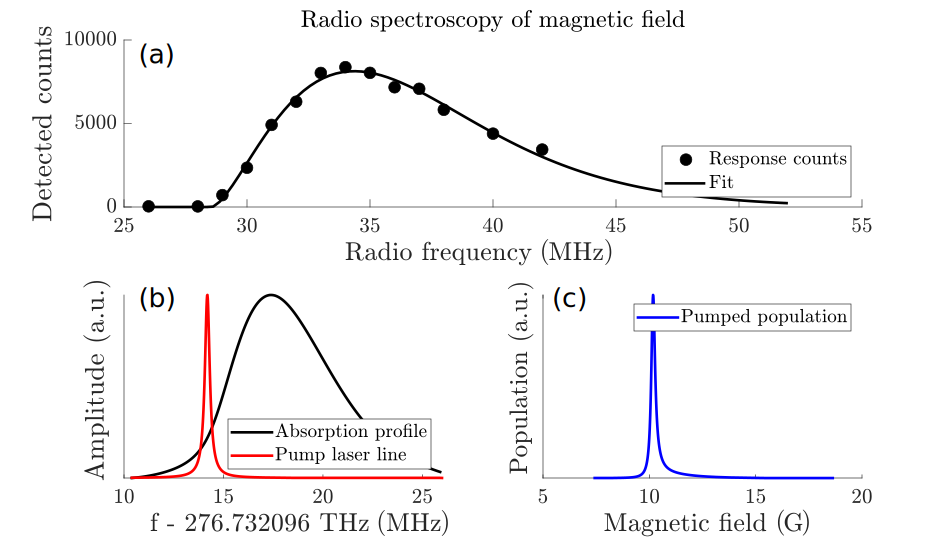
\includegraphics[width=\textwidth]{fig/spectroscopy/rf_spec_subfig}
  \caption{Determination of magnetic field for Zeeman shift correction.
	The number $n_\text{D}$ of atoms detected after probing the trap with 300 ms of RF radiation is shown in (a) versus the frequency of the applied radiation.
	Each point is an average of three shots.
	A Bose-Einstein fit models the population density $n_\text{T}$ of the $2\triplet S_1$ state at a given field strength.
	In (b) the calculated absorption profile of the gas in the vicinity of the 1083 nm pump transition is shown, along with the spectral profile of the pump laser. N.B. the frequency axis is in units of MHz, relative to the resonance as specified in THz.
	The pump laser selectively excites atoms with a certain Zeeman splitting, leading to a population of atoms in the $2\triplet P_2$ state (c) that is concentrated around a specific magnetic field strength.
	The resulting Zeeman broadening is dominated by the probe beam linewidth.}
  \label{fig:RF_spec}
\end{figure}


% \begin{figure}
% 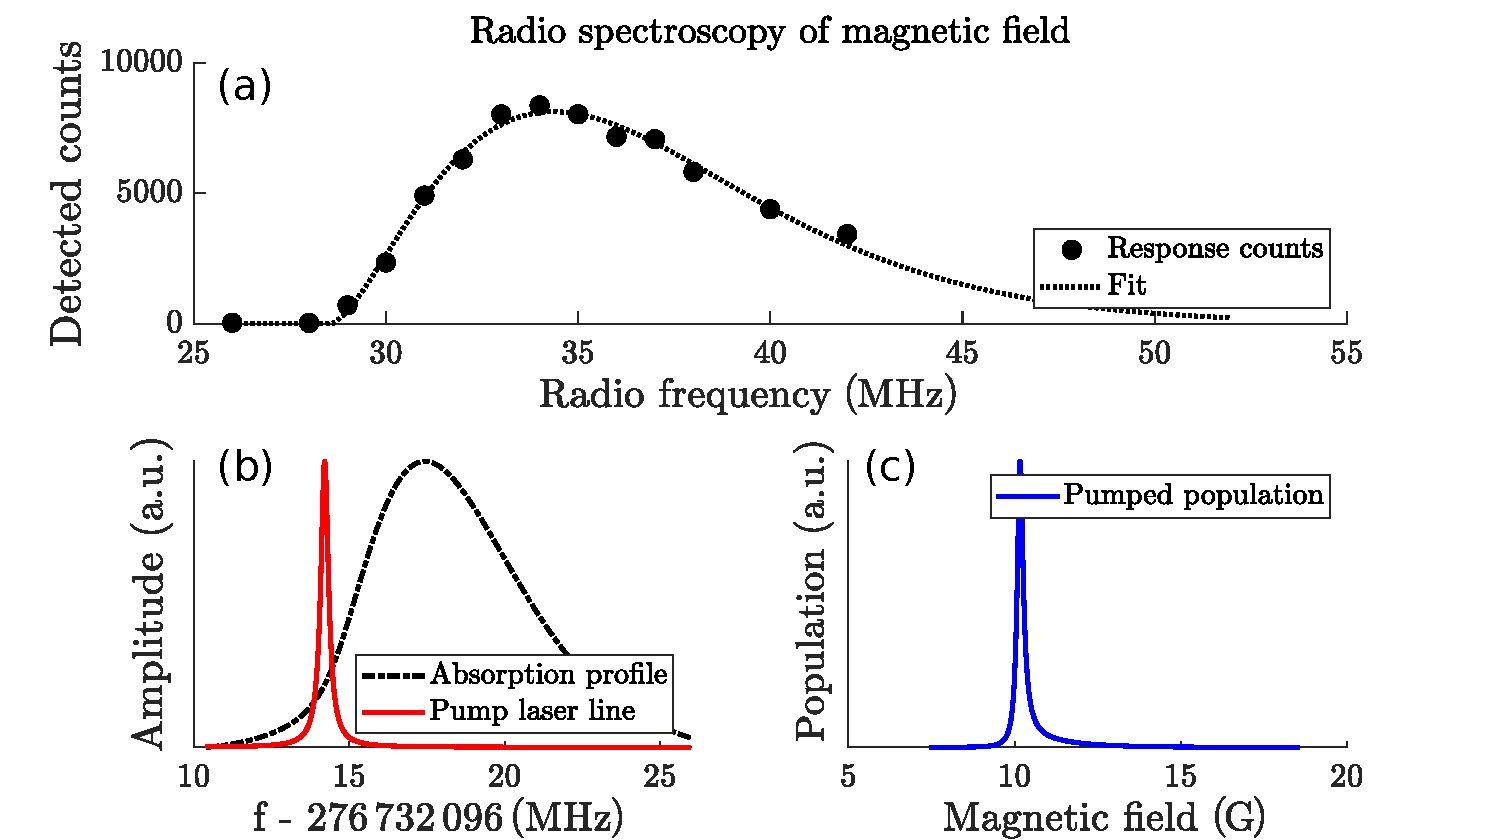
\includegraphics[width=0.5\textwidth]{fig/spectroscopy/rf_spec_subfig-eps-converted-to.pdf}
% \caption{Determination of magnetic field for Zeeman shift correction.
% 	The number $n_\text{D}$ of atoms detected after probing the trap with 300ms of RF radiation is shown in (a) versus the frequency of the applied radiation.
% 	Each point is an average of three shots.
% 	A Bose-Einstein fit models the population density $n_\text{T}$ of the $2\triplet S_1$ state at a given field strength.
% 	In (b) the calculated absorption profile of the gas in the vicinity of the 1083nm pump transition is shown, along with the spectral profile of the pump laser.
% 	The pump laser selectively excites atoms with a certain Zeeman splitting, leading to a population of atoms in the $2\triplet P_2$ state (c) that is concentrated around a specific magnetic field strength.
% 	The resulting Zeeman broadening is dominated by the probe beam linewidth.}
% \label{fig:RF_spec}
% \end{figure}

% The probe laser can only excite atoms pumped into the $2\triplet P_2$ state, which has a population distributed over a finite range of magnetic field strengths.
	% The peak of the response to the probe laser is given by the convolution of the probe laser spectrum and the density of pumped states over the magnetic field strengths.
	% We identify the 

% Finite temp in non-uniform field would lead to Zeeman broadening as well as a shift...
	% ungh run the trap sim?

	


\begin{figure}
  \begin{minipage}[t]{0.6\textwidth}
  \vspace{0pt}
  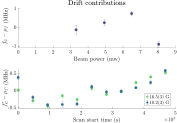
\includegraphics[width=\textwidth]{fig/spectroscopy/power-drift-combined}
  \end{minipage}\hfill
  \begin{minipage}[t]{0.38\textwidth}
  \vspace{0pt}
\caption{Top: Variation in fitted centre frequency for single scans across the $5\triplet D_1$ line versus applied laser power.
	The measurements at increasing beam power were not taken in chronological order Bottom: Variation in fit center frequency for the $2\triplet P_2 - 5\singlet D_2$ between scans.
	The value of the fitted peak centre $f_\textrm{c}$ is shown for each field strength, relative to the mean $\mu$ of all values for that field strength.}
\label{fig:power_drift_combined}
  \end{minipage}
\end{figure}



	Other precision measurements of transition frequencies have been shown to be subject to line pulling effects \cite{Marsman15,Marsman15PRA}.
	These effects arise in multilevel transitions because of interference between the laser-driven transition path and off-resonant driving through transitions with neighbouring intermediate states.
	The worst-case shift can be approximated by $w_{\text{pump}}^2/\Delta_{2P} + w_{\text{probe}}^2/\Delta_{5L}$ \cite{Marsman15,Marsman15PRA}, where the $w$ terms are the linewidths of the pump and probe transitions, and the $\Delta$ terms are the Zeeman splittings between the sublevels of the pump and target states.
	The largest estimate among all the reported transitions is 500 kHz.
	While this uncertainty is dominated by other effects in our experiment, it may be important to understand them for improved measurements in the future.
	% \com{I actually think this is bogus because we drove through (hyperfine) magnetic sublevels. For these, $\Delta\rightarrow 0$ at B=0, so the above expression would diverge, as oppsed to the case in Marsman \emph{et al} where they considered fine structure sublevels with $\delta>0$ at $B=0$. Without doing the calculations I suspect this rule of thumb doesn't actually apply to hyperfine levels but I'm not certain. Either way I will probably leave this in, as I'm unsure whether it's worth entering into that discussion.}

	There was no significant detectable contribution from the AC Stark effect.
	This can be seen in Fig.	\ref{fig:power_drift_combined}: The rightmost data point in the top panel was taken first, followed by the others in increasing order. Two conclusions are apparent: First, the center frequency drifted up during the course of the four scans, and second, that such drift dominated any effect the beam power has on the center frequency. We can characterize the time-dependent drift by examining the drift in center frequency over time with fixed beam power, as shown in the bottom panel, which depicts the individual results of each scan of the $5\triplet D_1$ transition. A drift on the order of 1 MHz per hour is seen, which is comparable to that found in the data shown in the top panel. Separately, after locking the spectroscopic laser system to the Cs reference transition, the inherent drift of the wavemeter can thus be determined, and explains the variation in centre frequency shown in Fig.	\ref{fig:power_drift_combined}.


	%  transition with varying probe beam powers, the dependence of the centre frequency on the laser power was dominated by the drift in the wavemeter output, as shown in Fig.
	% \ref{fig:power_drift_combined}.
	% For the triplet-singlet transition, the increase in laser intensity is more than compensated for by the reduced dipole matrix element, and hence the same conclusion follows.
	
	The noise floor is ultimately determined by two main factors: The variation in population of subsequent realizations of BEC (shot noise) and the Bernoulli process resulting from imperfect detection efficiency.
	The shot noise is by far the dominant noise process, with a standard deviation at the level of $\approx 10\%$, on the order of $5\times10^4$ atoms in the worst case. 
	For comparison, the relative error induced by imperfect detection can be modeled as a Bernoulli process. 
	Assuming a detection efficiency of $\eta=8\%$, the respective relative error is given by $\sqrt{\textrm{Var}_N}/N=\sqrt{N\eta(1-\eta)}/N\approx0.86/\sqrt{N}$, where $N$ is the atom number, which is below 1\% for the largest clouds. 
	The large-$N$ limit determines the noise floor as the signal is calculated by the relative difference between measurement (probe-on) and calibration (probe-off) shots.
	It should be noted, then, that an improvement in the precision of the number detection would not lead to a consequential reduction in the noise floor, as it is the underlying shot noise itself that is the limiting factor.
	Therefore there is no distinct advantage of using either the MCP-DLD detector or optical absorption imaging, as the latter can also obtain sub-percent precision in single shots \cite{Ockeloen10}.


\section{Discussion}

	This chapter described multilevel laser absorption spectroscopy of excited state transitions in ultracold helium.
	The observations include the first observation (to my knowledge) of the forbidden $2\triplet P_2 - 5\singlet D_2$ transition.
	These measurements agree with current predictions within the error budget and suggest that the $93\sigma$ difference between previous measurements \cite{Martin60} and predictions \cite{Morton06} of the $\PStateManifold_2  -  \UpperS$ and $\PStateManifold_2  -  \SpecUpperStateManifold$ intervals are due to an unknown systematic error\footnote{As a historical note on the advancement of experimental methods, Martin's measurements were made using a nitrogen-cooled helium discharge lamp fed through an in-vacuum prism onto photographic plates, on which the line separations were measured by hand with a ruler.}.
	This work offers five contributions to the NIST database of atomic spectral lines.

	The techniques described here are readily extensible to other opportunities in $^4$He structure measurements.
	For example, while there is an outstanding 7.4$\sigma$ disagreement between the predicted and observed singlet-triplet interval for the n=3 level in $^3$He \cite{Morton06,Derouard80}, the corresponding transition in $^4$He has never been directly measured.
	An indirect measurement in $^4$He could be made with the techniques described here by taking the difference betweeen the $2\triplet P_2 - 3\triplet D_2$ and $2\triplet P_2 - 3\singlet D_2$ transitions near 587.6 nm and 587.4 nm.
	While the latter transition is also spin-forbidden, it is predicted to be an order of magnitude stronger than the $2\triplet P_2 - 5\singlet D_2$ transition reported here \cite{Morton06}.

	{Further, energies of other $2L-nD$ transitions in $^4$He are a few MHz larger than predicted, apparently independent of $L$ \cite{Wienczek19,Yerokhin20}.
	The results here deviate from this trend, and invite independent verification.
	Further study of transitions between states from different shells to MHz precision or better, in particular the prospective study of the $2\triplet P - 3 D$ intervals, would also provide further clarification.}

	% For instance, the hypothetical $10/n^3$ MHz shift could be checked by a measurement of the $2~P-n~D$ transitions accurate to sub-MHz precision.
	Simply exchanging the light source would suffice to make these measurements, but a definitive comparison with theory would require an improved frequency reference.
	The associated theoretical uncertainties are dominated by the 700 kHz uncertainty in the lower state \cite{Pachucki17,Wienczek19}.
	As the $\alpha^7$ terms could improve the theoretical accuracy to as little as 10 kHz \cite{Pachucki17}, this more challenging precision appears to be a more appropriate budget, and readily achievable with current methods.
	
	Reference-locked optical frequency combs can readily achieve kHz accuracy or better \cite{Luo15,Rengelink18}.
	The comb would need to be integrated in a similar technique to that in Ref. \cite{Rengelink18}, which achieved a 200 Hz uncertainty in their measurement of the $2\triplet s_1 \rightarrow 2\singlet S_0$ transition.
	In a suitable setup, a reference-locked comb would be used in a phase-locked loop to transfer-lock the probe light, or at least light that could be fed into a doubling cavity.
	Such an upgrade would eliminate the systematic uncertainties due to the wavemeter, Cesium cell, and probe lock loop.
	It would also be prudent to replace the RF driver on the pump beam AOM, whose RF linewidth was on the order of 300 kHz, with an oscillator of comparable quality to that in the probe AOM (with a 1 Hz linewidth, as is also used in the main cooling laser lock).
	The next leading uncertainty is associated with and Zeeman effect.
	Magnetic field strengths can be determined by RF spectroscopy with sub-kHz accuracy and so would not present a serious limitation.
	One could also consider illuminating a trapped cloud with an exceptionally weak pump beam on resonance, and scan the probe beam across the target transition while measuring the difference in heating rate (similar to our measurement of the  427 nm forbidden transition \cite{Thomas20}), without using the evaporative cooling ramp. 

	Extending these methods to direct measurements on $^3$He would also permit isotope shift measurements from forbidden excited-state transitions in $\triplet$He.
	Theoretical calculations of isotope shifts are already accurate to the sub-kHz level, so such measurements would be even more demanding than the prospects above.
	Existing demonstrations of comparable accuracy \cite{Rengelink18} show such measurements are worthy challenges whose completion can access nuclear structure information at the femtometre scale via optical atomic spectroscopy.


\vfill

\begin{flushright}
\singlespacing
\emph{
``Immediately you would like to know where this \\
number for a coupling comes from: is it related to pi\\
or perhaps to the base of natural logarithms? \\
Nobody knows.\\
It's one of the greatest damn mysteries of physics: a magic number \\
that comes to us with no understanding by man. You might say \\
the ``hand of God" wrote that number, and ``we don't know how\\
He pushed his pencil." We know what kind of a dance to\\
do experimentally to measure this number very accurately,\\
but we don't know what kind of dance to do on the computer\\
to make this number come out, without putting it in secretly!"}\\
- Richard P.
Feynman \footnote{\emph{QED: The Strange Theory of Light and Matter}.
	Princeton University Press.	p.	129.	(1985)}
\end{flushright}
\onehalfspacing
